\section{Preserved Development Evidence and Diagnostics}
\label{app:development-v13}
These are the pre-v14 development analyses on their original supports. Fixed-fit
intervals and their simulation validation do not validate the FACED joint bootstrap.

\subsection{Evaluation coverage}
% evidence: paper/generated/final_closure_v9/verification/verification.json; configs/final_robustness_v9.json
We evaluate EmoEEG-MC (30 eligible participants, 42 stimuli; valence and
arousal) and Urban Appraisal (62 participants, 56 street images; genuine
valence trials only) \citep{openneuro_ds005540,openneuro_ds006850}.
Deterministic identity blocks test every eligible participant and stimulus once,
yielding 252 and 695 fixed test trials. The design tests five diagonal blocks,
not every possible participant--stimulus pair. Urban is an external appraisal
task, not an identical replication of emotion induction, and neither dataset is
an untouched confirmatory cohort.

Each task includes band-power Ridge, frozen LaBraM, and standard Braindecode
EEGNet \citep{jiang2024labram,lawhern2018eegnet}. Two bounded settings per model,
five identity blocks, and all 25 dose cells yield 1,500 model-cell results; these
cells are not independent observations. Ridge settings vary the candidate
regularization grid, while EEGNet settings vary learning rate. Validation
selects hyperparameters and training duration. Population refitting uses
training and validation trials but never test or calibration trials. We record
200 nonconstant EEGNet selection/refit histories as execution evidence, not as
proof of optimization. The Appendix reports full preprocessing, coverage,
budgets, and historical model panels.

% evidence: paper/generated/reviewer_revision_v12/learning_diagnostics.csv
The archived records show that, among 50 direct and 50 residual EEGNet fits per
task, 12/10 Emo and 8/7 Urban fits select epoch one; median selected epochs are
18/17.5 and 11/7.5. Training objectives decrease in the median for all four
groups. This rules out every network remaining at its initial fit, but does not
establish optimal tuning or a positive held-out EEG signal.

\subsection{A favourable total gain need not be an EEG gain}
\begin{table}[t]
\centering\small
\caption{Changing the comparison at the predeclared maximum dose $(p,s)=(8,8)$. Total system gain $EC-P$ includes the EEG-free calibration gain $PC-P$. The last column is the paired percentile interval for $EC-PC$, not a difference of interval endpoints. These descriptive endpoints do not replace the primary uniform-grid mean.}
\label{tab:resource-decomposition}
\begin{tabular}{@{}llrrrl@{}}
\toprule
Task & Setting & $EC-P$ & $PC-P$ & $EC-PC$ & Paired interval \\
\midrule
EmoEEG-MC & Band-power R1 & +0.1312 & +0.1420 & -0.0108 & [-0.0429, +0.0219] \\
EmoEEG-MC & Band-power R2 & +0.1318 & +0.1420 & -0.0102 & [-0.0403, +0.0206] \\
EmoEEG-MC & LaBraM R1 & +0.0961 & +0.1420 & -0.0459 & [-0.1098, +0.0139] \\
EmoEEG-MC & LaBraM R2 & +0.1325 & +0.1420 & -0.0095 & [-0.0419, +0.0243] \\
EmoEEG-MC & EEGNet L1 & +0.1400 & +0.1420 & -0.0020 & [-0.0065, +0.0027] \\
EmoEEG-MC & EEGNet L2 & +0.1420 & +0.1420 & 0.0000 & [-0.0040, +0.0043] \\
Urban & Band-power R1 & +0.0639 & +0.0774 & -0.0135 & [-0.0561, +0.0362] \\
Urban & Band-power R2 & +0.0643 & +0.0774 & -0.0131 & [-0.0398, +0.0199] \\
Urban & LaBraM R1 & +0.0587 & +0.0774 & -0.0186 & [-0.0563, +0.0126] \\
Urban & LaBraM R2 & +0.0689 & +0.0774 & -0.0085 & [-0.0373, +0.0172] \\
Urban & EEGNet L1 & +0.0885 & +0.0774 & +0.0111 & [-0.0147, +0.0360] \\
Urban & EEGNet L2 & +0.0851 & +0.0774 & +0.0078 & [-0.0064, +0.0252] \\
\bottomrule
\end{tabular}
\end{table}

% evidence: paper/generated/evidence_argument_v10/decomposition_maximum_dose.csv
Table~\ref{tab:resource-decomposition} applies the same predeclared maximum dose
to every setting. For EmoEEG-MC LaBraM R1, $EC$ improves on the uncalibrated
prior $P$ by $+0.0961$. Yet the same calibration labels improve the EEG-free
predictor by $+0.1420$, leaving a matched EEG difference of $-0.0459$
$[-0.1098,+0.0139]$. In Urban, the corresponding quantities are $+0.0587$,
$+0.0774$, and $-0.0186$ $[-0.0563,+0.0126]$. The system-level point gains are
positive; the EEG-specific contrasts are not established as positive. This is
the judgement that resource matching changes.

\begin{table}[t]
\centering\small
\caption{Primary uniform-grid mean matched EEG increment in CCC, with two-sided 95\% five-block $t$ intervals (df=4). Each task averages five fixed identity blocks and all 25 dose cells. Settings are sensitivity checks, not independent replications.}
\label{tab:primary-v13}
\begin{tabular}{@{}lll@{}}
\toprule
Setting & EmoEEG-MC: mean [interval] & Urban: mean [interval] \\
\midrule
Band-power R1 & -0.0069 [-0.0464, +0.0327] & -0.0060 [-0.0631, +0.0511] \\
Band-power R2 & -0.0091 [-0.0409, +0.0226] & -0.0069 [-0.0444, +0.0307] \\
LaBraM R1 & -0.0320 [-0.0883, +0.0242] & -0.0173 [-0.0607, +0.0261] \\
LaBraM R2 & -0.0137 [-0.0492, +0.0219] & -0.0035 [-0.0312, +0.0242] \\
EEGNet L1 & -0.0001 [-0.0065, +0.0064] & +0.0073 [-0.0117, +0.0264] \\
EEGNet L2 & +0.0003 [-0.0046, +0.0052] & +0.0086 [-0.0094, +0.0265] \\
\bottomrule
\end{tabular}
\end{table}

% evidence: paper/generated/final_revision_v13/block_t/table_added_value_summary.csv
The primary full-grid summaries in Table~\ref{tab:primary-v13} tell the same
bounded story: all 12 task--setting block-$t$ intervals include zero. The
conclusion is unchanged under released percentile, basic, and earlier t-normal
sensitivities. No equivalence margin was prespecified, so this does not establish
equivalence, universal reversal, absence of EEG information, or a ceiling on
future EEG methods. The secondary MAE contrast for LaBraM R1 indicates increased
error in both tasks under the primary construction; other configurations are
uncertain or interval-sensitive. Appendix~\ref{app:latest-evidence} reports all
CCC and MAE settings rather than selected rows.

% evidence: paper/generated/final_revision_v13/sensitivity/sensitivity_summary.json
Post-primary checks preserve that interpretation. An alternative identity
partition and complete refit shifts any point estimate by at most 0.0135 (Emo)
or 0.0154 (Urban), with all 12 intervals covering zero. Across three EEGNet
initialization schedules at the four resource corners, all 12 task--setting--run
intervals cover zero and the largest point span is 0.0097. Last-block LaBraM
residual fine-tuning gives $-0.0110$ [$-0.1041,+0.0820$] and $-0.0404$
[$-0.1159,+0.0351$]. These are bounded sensitivities run after the primary
analysis, not independent cohorts or an unconditional retraining interval.

% evidence: paper/generated/reviewer_revision_v12/figure_manifest.json
\begin{figure}[tp]\centering
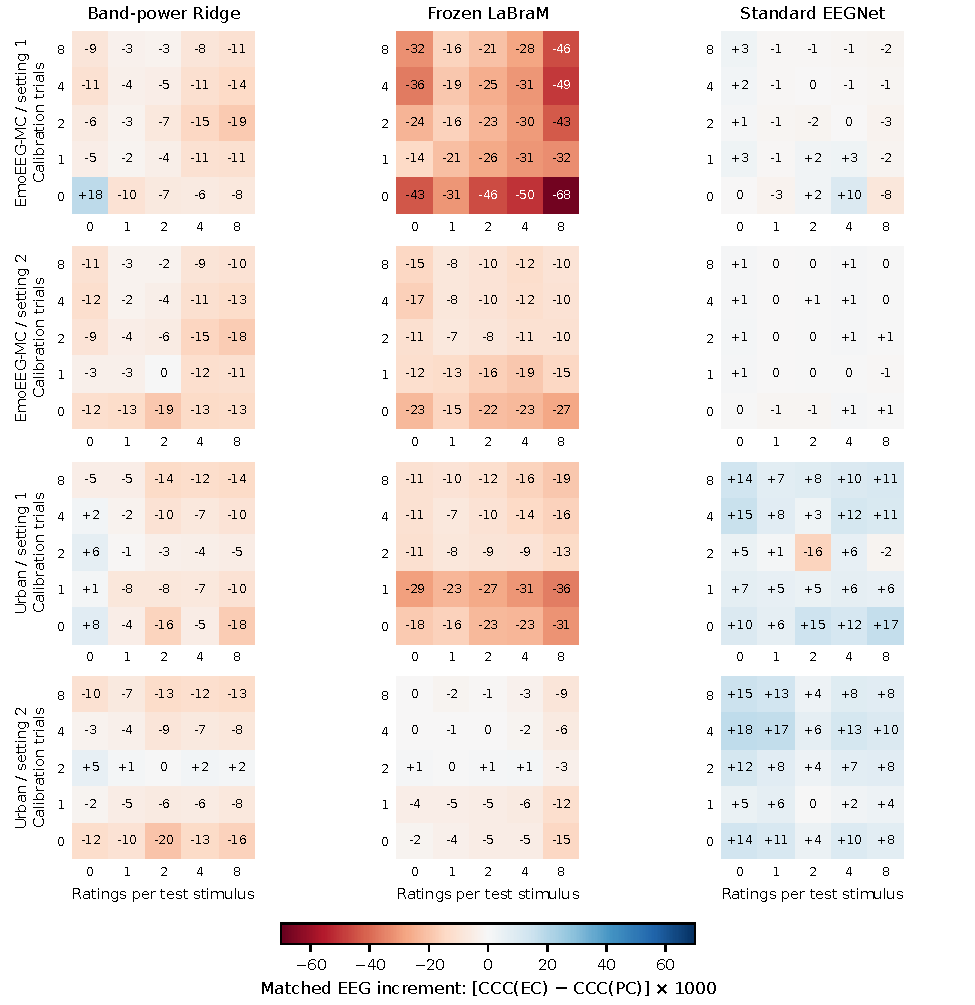
\includegraphics[width=\linewidth]{../generated/reviewer_revision_v12/matched_increment_heatmap.pdf}
\caption{All 12 matched-increment grids, with every dose retained. Entries and
color scale are $1000\Delta_{\rm EEG}$; rounded zero is not exact equality.
Rows distinguish tasks and settings (R1/L1, R2/L2); columns distinguish model
families. Positive values favor EEG. Each value averages five block-level
paired CCC contrasts. This is a descriptive display of already inspected
data, not an additional confirmatory test. Conditional pointwise stability
ranges and within-model dose-family bands accompany every cell in the released CSV.}
\label{fig:matched-grid}
\end{figure}

% evidence: paper/generated/reviewer_revision_v12/heterogeneity_summary.json
Figure~\ref{fig:matched-grid} exposes heterogeneity hidden by the uniform mean.
For example, Urban EEGNet L2 has positive point estimates in every cell, ranging
from $+0.0003$ to $+0.0177$; these do not establish positive increments at the
reported precision. None of the 300 cells has a positive pointwise CCC
range. Two Urban LaBraM R1 cells have negative pointwise ranges, but
neither survives its within-model dose-family band. These ranges are descriptive
because the cell estimands failed full calibration. We retain all 48
task--setting--corner comparisons $(0,0),(8,0),(0,8),(8,8)$ in a separate table;
no cell selection or averaging of interval endpoints is used.

% evidence: paper/generated/final_closure_v9/normal_t/table_added_value_summary.csv
Why is the matched comparator material? From zero dose, eight target-user
calibration trials increase EEG-free $PC$ CCC by $+0.2036$ in EmoEEG-MC and
$+0.1564$ in Urban. Eight other-participant ratings per test stimulus increase
it by $+0.4907$ and $+0.3408$, respectively; both interval constructions are
positive. The fact that labels help is unsurprising. Their magnitude relative
to the matched EEG contrasts shows why unequal label access can change the
attribution attached to a system score.

\subsection{Uncertainty and evaluator validity}
% evidence: paper/generated/final_closure_v9/percentile/added_value_statistics.json; paper/generated/final_closure_v9/normal_t/added_value_statistics.json
The crossed bootstrap applies identical participant and stimulus
multiplicities to every paired predictor, cell, and block. Of 2,000 draws, 1,985
are valid for EmoEEG-MC and 2,000 for Urban. The primary two-sided 95\% interval uses the
crossed-bootstrap standard error and a $t_{4}$ critical value because the final
estimand averages five predeclared identity blocks. Percentile, basic, and the
earlier within-block t-normal constructions are sensitivity checks. Every
construction conditions on fitted predictions and omits retraining uncertainty.
Pointwise ranges and separately released dose-family bands do not support
calibrated cell selection or all-model multiple comparisons.

% evidence: paper/generated/final_closure_v9/percentile/added_value_statistics.json
The relevant cluster sizes are those within each scoring block: Emo has six
participants and eight or nine stimuli per block; Urban has 12 or 13
participants and 11 or 12 stimuli. The whole-dataset participant count does
not by itself validate a mean of small-block CCCs. We therefore distinguish
the earlier single-block simulations below from the topology-matched
five-block check in Appendix~\ref{app:revision-diagnostics}.

% evidence: results/block_t_validation_v13/summary.csv; results/block_t_validation_v13/completion.json
The new topology-matched validation executes 300 replicates for each of four
Gaussian scenarios per task, with 2,000 bootstrap draws and no failed runs.
For the primary uniform mean, block-$t$ coverage is 0.993 for Emo and 1.000
for Urban under trial signal, and 0.980 and 0.983 under participant-constant
signal; the two non-signal checks cover at 1.000. The corresponding Wilson
Monte Carlo lower bounds are 0.957--0.987. The minimum cellwise coverage is
still 0.917, so this validation supports only the predeclared uniform mean.
The block-$t$ correction was introduced after the earlier interval diagnostics
failed, but its critical value follows the five-block aggregation and does not
use the observed EEG effect signs or magnitudes. Its evidence remains limited
to these four Gaussian families. We therefore make no calibrated cellwise,
equivalence, or unconditional retraining claim. Earlier single-block tests in
Appendix~\ref{app:evaluator-validation} cannot widen that scope.

\subsection{Scope checks and retained negative evidence}
Earlier EmoEEG-MC and MusicEEG surfaces, compact versus standard EEGNet,
CBraMod, LaBraM random controls, frozen EMOD, and calibration variants remain in
Appendix~\ref{app:exposure-surface}. They use distinct supports or protocols and
are not replications of the primary grid. The earlier MusicEEG LaBraM mean
increment is $\VThreeMusicMean$ [$\VThreeMusicLow,\VThreeMusicHigh$], an
uncertain auditory result that we retain rather than omit. Resource-conditioned
model selection likewise has no stable mean CCC benefit
(Appendix~\ref{app:selection-utility}).

Identity probes and subspace perturbations are representation diagnostics, not
causal evidence. The ds006866 analysis concerns condition exposure because
image identity is unavailable. DENS is missingness-limited; SEED-V is an
authorized aggregate supplement, not an openly redistributed benchmark. The
repaired EMOD single-seed check is neither a full original-task reproduction nor
evidence against EMOD, and mdJPT has no completed numerical audit here. These
records bound model and domain coverage; none is promoted to primary evidence.

